\documentclass{beamer}

\usepackage[utf8]{inputenc}
\usepackage[french]{babel}

\begin{document}

\author{A}
\title{B}
\date{C}

\begin{frame}
  \titlepage
\end{frame}

%%% 1 EMC
\begin{frame}{}

\end{frame}

\begin{frame}{}

\end{frame}

\begin{frame}{}

\end{frame}

\begin{frame}{}

\end{frame}

\begin{frame}{}

\end{frame}


%%% 2 DLX
\begin{frame}{}

\end{frame}

\begin{frame}{}

\end{frame}

\begin{frame}{}

\end{frame}

\begin{frame}{}

\end{frame}

\begin{frame}{}

\end{frame}



%%% 3 ZDD
\begin{frame}{}

\end{frame}

\begin{frame}{}

\end{frame}

\begin{frame}{}

\end{frame}

\begin{frame}{}

\end{frame}

\begin{frame}{Réduction vers EMC}
  \begin{columns}
    \column{0.5\textwidth}

  \begin{displaymath}
   \left(\begin{array}{ c c c c c }
   1 & 0 & 1 & 1 \\
   0 & 1 & 1 & 0 \\
   1 & 1 & 0 & 1 \\
   1 & 0 & 0 & 1 \\
   0 & 1 & 0 & 0
  \end{array}\right)
  \end{displaymath}

    \column{0.5\textwidth}
    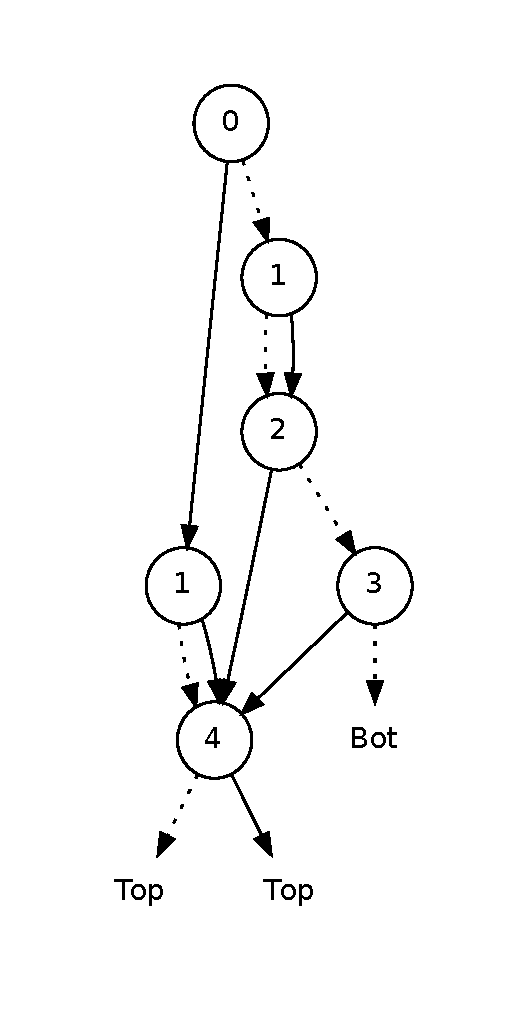
\includegraphics[height=0.9\textheight]{../column.pdf}
  \end{columns}
\end{frame}

\begin{frame}{Réduction vers EMC}
  \begin{columns}
    \column{0.3\textwidth}

  \begin{displaymath}
   \left(\begin{array}{ c c c c c }
   1 & 0 & 1 & 1 \\
   0 & 1 & 1 & 0 \\
   1 & 1 & 0 & 1 \\
   1 & 0 & 0 & 1 \\
   0 & 1 & 0 & 0
  \end{array}\right)
  \end{displaymath}

    \column{0.7\textwidth}
    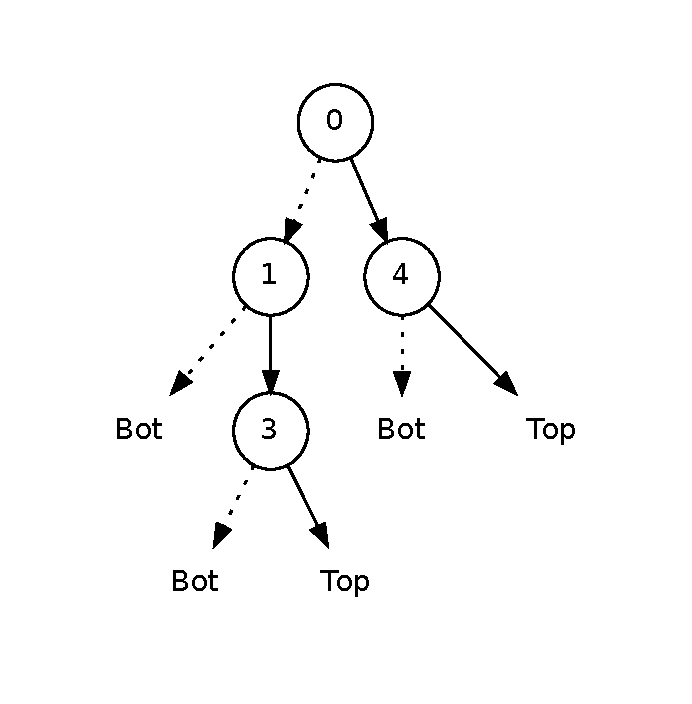
\includegraphics[height=0.8\textheight]{../inter.pdf}
  \end{columns}
\end{frame}



%%% 4 bibliothèque OCaml
\begin{frame}{}

\end{frame}

\begin{frame}{}

\end{frame}

\begin{frame}{}

\end{frame}

\begin{frame}{}

\end{frame}

\begin{frame}{}

\end{frame}


\begin{frame}{Conclusion}
  
\end{frame}

\end{document}
